\documentclass[../main/main.tex]{subfiles}

\newdate{date}{01}{04}{2020}

\begin{document}

\section{Lecture 7}
 \displaydate{date}. Compiled:  \today. Alice.

\subsubsection{Slide 105}

\begin{figure}[h!]
\centering
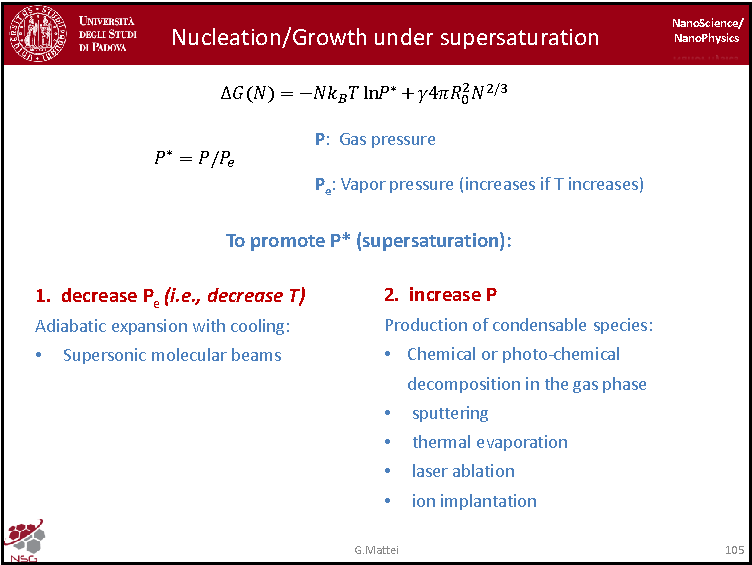
\includegraphics[page=1,width=0.9\textwidth]{../lessons/pdf_file/7_lesson.pdf}
\end{figure}

In this lesson we go on with the description of the process of nucleation and growth of supersaturated solution. In the previous section we have seen the concept of Gibbs equation and the definition of the supersaturation degree as the ratio \( P^*=P/P_e \) (between the gas pressure and vapor pressure at that specific temperature). The volume contribution to the Gibss free energy in the creation of a stable nuclei of the precipitating phase can be proportional to \( \ln{P^*}  \). On the contrary, the surface term of the variational Gibbs free energy is positive and tends to destabilize (it will dominate at smaller values), while the first dominate at larger values of the values (or for number of atoms in the precipitating phase).
Altough, we have developed this theory for precipitation from vapor phase to a liquid phase, all those concept can be really trasferred to solid state. We can use the same concept of gas pressure in a solid phase by resorting to the equivalent concept which is the concentration. We were describing the simple homogeneous nucleation that is a nucleation which is not a system by defect, which involves just pure phases. We can divide the number of strategies that we have to promote the nucleation growth of precipitating phase by controlling (at a given temperature) the ratio \( P^* \). To control this ration we have two possible approaches:
\begin{enumerate}
\item If we want to increase \( P^* \), we have to decrease the denominator \( P_e \), which is a function of temperature (hence, to decrease it we have to decrease \( T \) temperature of the environment). Among the different techniques brifely mentioned in the previous lessons which can be used to synthesize nanostructured material, not so many are dealing with this kind of approach in which we decrease the temperature \( T \). One technique is the \textbf{supersonic molecular beams}, which is a techinique which exploit an adiabatic expansion which promote cooling of a gas carrier to precipitate the nanoparticle in a chamber.

\item The vast majority of techinques works on the numerator of \( P^* \), which consists in increasing \( P \).
We just add more material in the gas, or more atom in the solid matrix to promote nucleation and growth. In practice, on this approach are based most of the techniques we describe in this course as \textbf{ion implantation} (produce nanoparticle in a glass). Normally all the bottom up techniques are working with this kind of approach (as \textbf{thermal evaporation}, \textbf{sputtering}, \textbf{chemical and physical vapour deposition} and so on).

\end{enumerate}

\newpage

\subsubsection{Slide 106}

\begin{figure}[h!]
\centering
\includegraphics[page=2,width=0.9\textwidth]{../lessons/pdf_file/7_lesson.pdf}
\end{figure}

Let us give an hint in how the first technique works: the one which decrease the temperature to promote the increase of the supersaturation. In this scheme we have a sketch of the apparatus normally used for this kind of experiment.

We have an initial chamber in which we put the gas that we want to condensate at a given temperature \( T_0 \) and pressure \( P_0 \). We can let the gas in the initial chamber in another chamber in which we have made vacuum with a pump. The gas expands in this chamber through a nozzle to control the diameter which controls basically the dinamics of the effusive movement of the atoms in the chamber according to the fact that the diameter of the nozzle is less of the mean free path of the particles (\( d < \lambda  \)). If \( d > \lambda  \) we have a supersonic beam expansion. What is important is that since in this chamber we evacuate the space through the pump there is a reducation in the temperature because we have a sort of adiabatic expansion, physically controlled by adiabatic trasformation and descrbibed by the simple equation of the perfect gas.

\newpage

\subsubsection{Slide 107}

\begin{figure}[h!]
\centering
\includegraphics[page=3,width=0.9\textwidth]{../lessons/pdf_file/7_lesson.pdf}
\end{figure}

You may remember that an adiabatic expansion involves the equation
\begin{equation*}
  P V^ \gamma = const, \quad \gamma \equiv \frac{c_P}{c_V}  >1
\end{equation*}
 where \( c_P \) is the specific heat at constant pressure and \( c_V \) at constant volume. If we rearrange the terms in the above equation considering the perfect gas equation we can recast the entire equation in term of pression and temperature. If we label the constant as the initial value of the quantity on the left hans size, we can rewrite very simpli the evolution of the temperature of the gas as a function of the initial temperature and pressure accorduing to the final pressure \( P \). If we start from \( P < P_0 \), also the temperature will decrease. Those are simple plots in the case of monoatomic an biatomic perfect gas equation. We see how the temperature decrease with the pressure.

 This decrease promotes locally the supersaturation, so we can obtain nanoclusters during the flight of the expanding beams. In order to reach a better homogeneous temperature in the system the precipitating phase  (gas) is also assisted by a gas carrier (an inner gas like argon, which aim is just promote thermal equilibration through collisions between atoms and to confine the movement of the atoms within a prescribed path as we have seen in the expansion chamber in the previous slide).

 Of course we can complicate a lot
(\textbf{Slide 106}) this very simple system just adding a mass spectrometer or additional slits so that we can collimate the beam to be deposited into a target and we can have a mass selected deposition of nanoclusters in our samples or we can add spectrometer to measure during the flight of formed cluster and investigate their nature (as for instance optical and spectroscopy). By the way this techinque is one of the first used for producing the first metallic nanoclusters. People were able to see that there was a remarkable stabilization of specific size of number of atoms per nanoparticles which is a biproduct of the stabilization of the electronic structure as a function of the number of atoms.


Just to get back to the (\textbf{Slide 107}) technique, of course we can for instance increase the cluster density by:
\begin{itemize}
\item  increasing the initial pressure \( P_0 \);
\item  increasing the diameter of the nozzle \( d \);
\item decreasing the initial temperature \( T_0 \). So we start to have a lower temperature in the initial chamber that nucleation will be promoted.

\end{itemize}


However, this techinque is quite peculiar among the techinques with bottom/up approach it involves the decreasing in the temperature such that the vapor pressure decrease and we can increase supersaturation for a given number of atoms in the system.

\newpage

\subsubsection{Slide 108}

\begin{figure}[h!]
\centering
\includegraphics[page=4,width=0.9\textwidth]{../lessons/pdf_file/7_lesson.pdf}
\end{figure}

Now, we describe in more detail and to compare it with experimental activity, the nucleation and growth process as a function of two variables, time for a given temperature and as a function of the temperature. How can we use both variables to have a full control of precipitation process? We will try to use as a template, for verifying the concept that we have introduced in the previous part of this lesson, a solid state solution just to more clearly show that all the concept introduced for the basic very simple homogeneous nucleation vapor phase can be translated to the solid state just simpli changing pressure with concentration
and the concept of vapor pressure (equilibrium pressure) with the solubility limit.

\newpage

\subsubsection{Slide 109}

\begin{figure}[h!]
\centering
\includegraphics[page=5,width=0.9\textwidth]{../lessons/pdf_file/7_lesson.pdf}
\end{figure}

Just to understand what we would like to describe when we mention temperal evolution of the system under nucleation and growth.
Suppose we have the time evoling in this direction, the steps are:
\begin{enumerate}
\item Nuclei formation, we need to have a supersatured solution.
In the end we can obtain:
\begin{itemize}
\item an average radius of the particles, which is the \textbf{critical radius} \( R^* \), connected to the basic thermodynamic quantities:
\begin{equation*}
  R^* = \frac{2 \gamma  }{\Delta g_V}
\end{equation*}
where the \( \gamma   \) is the surface extension that is the reversible work that you need to do to create a unit surface in our system. We have to be careful, because altough we use an homogeneous nucleation we will work in real world application were defects are always present and in particle since we are dealing with ion implantation, which is a rough technique in terms of damage it produces in the substrate of course a lot of defects are created and so we are dealing with an heterogeneous nucleation.

The basic difference is that we can safely assume that the basic input quantities as the critical radius \( R^* \) is the same but we just decrease the barrier of the energy we need to stabilize and growth the nanostructure.
Hence, we can safely assume all the concept of the homogeneous nucleation that we have described so far.

\item As time goes by, the second step is that when stable nuclei are formed we want to growth them. We are on the side of the variation of the Gibbs free energy where the volume contribution stash to dominate. Of course, if we have a sufficient degree of supersaturation, we described the initial process in which the supersaturation is still very high so there is an independent growth of each nanoparticle and the expenses of the atoms in the environment.  Basically, we have what is called a \textbf{diffusion limited aggregation} (DLA), a growth of the particle which is just controlled by diffusive process in vapor or in a solid. If we have an isolated system in which we set the total number of precipitating atoms in our system, as time goes by we will have a decreasing in the supersaturation degree, because atoms enters the stable nuclei and forms nanoparticles and we will see that the kinetic of the growth of the average radius of the system follow this equation:
\begin{equation*}
  R^2 (t) = R_0^2 + K_1 D t
\end{equation*}
the square of the radius as a function of time is directly proportional to the time thorugh the diffusion constant of the diffusing species of that particular matrix (either gas or solid).
The initial value is the radius at time zero of this evolution \( R_0 \).

In this regime all the clusters behave independently, so we can use the independent particle approach to describe the evolution.
This equation is quite intuitive, because it resemble the typical diffusive process in which we have the spatial coordinate is basically proportional to the square root of time (as Brownian motion in random walk).
When this process of diffusion limited aggregation starts to decrease the supersaturation and when the supersaturation is faling down we can basically enter in the new process.

\item Coarsening (or Ostwald ripening) stage. We have a competitive growth. Since nucleation is a statistical process we do not have a monodispersed system, so we will have a size dispersion. We will have clusters with different size and at that moment the Gibbs-Thomson equation starts to dominate to control the growth. In this case as we have seen we will have a competitive growth, that is the number of clusters in our system will decrease as a function of time. Basically, the smaller clusters dissolve and the atoms will increase the concentration in the system and after this stage they will feed the larger clusters growth. We have an increasing in size of the most stable larger clusters which are thermodynamically most stable than the smaller one.
In this case the \textbf{Gibbs-Thomson equation} is the equation that control the process and we will see that the temperal evolution of the redius follows this kinetic here:
\begin{equation*}
  R^3(t) = R_0^3 + K_2 D t
\end{equation*}
that is the cube of the radius as a function of time proportional to the time.

\end{itemize}


\end{enumerate}

Let us see how we can obtain with reasonable approximation an analytic solution of the time evolution of the radius in these two regimes that is the diggusion limited aggregation and coarsening. Moreover, how we can obtain expression for \( K_1 \) and \( K_2 \) constant.

We assume of course that nuclei formation has been occurred and we will start first with DLA process in which we have a large degree of supersaturation.

\newpage

\subsubsection{Slide 110}

\begin{figure}[h!]
\centering
\includegraphics[page=6,width=0.9\textwidth]{../lessons/pdf_file/7_lesson.pdf}
\end{figure}

To obtain this simple description we use a very simple balance between the number of atoms which enter the nanoparticle (which will promote the nanoparticle growth) and the number of atoms which goes out of nanoparticle. Of course, what is the engine which control alle the process? it is the starting concentration that we put in our system. Suppose that we have a solid matrix we will use the concept of concentration instead of pressure. Since we are dealing with a large degree of supersaturation and mentioned that we can resort to the independent particle approximation (in this process there is no competion between nanoparticle because of the large supersaturation, there are a large of atoms available that feed the nanoparticles). To solve analitycally the problem is not  sraight forward, because there is the moving boundary condition problem. The boundary is the surface of the nanoparticle.

Let us consider a radial coordinate system (homogeneous environment and all the part are supposed to be independently so we can set an origin of our system in the center of the growing nanoparticle), hence the 3d coordinates are recasted in an one dimensional system.

The concentration of the atoms in the precipitated phase (solid in this case) is the value \( c_P \), that is the numeric density of this phase (number of atoms per unit volume of that specific element that we want to growth, it is a known parameter) . The initial concentration of the atoms putted in our matrix is \( c_S \), which is an homogeneous value all around the particles. When the particles start to growth this value will be deplited with the rate which is high close to the surface of the nanoparticles and tends to zero at infinity distance from the nanoparticles.
So at very large distance from the center of nanoparticles we will have the initial value of the concentration and then we will have a decrease of the initial concentration toward the surface until a value called \( c_e  \) which is the concentration in the matrix with which the solid solution is in equilibrium with. It is the equivalent of vapour pressure in the case of liquid and vapor phases. We need to put \( c_s>c_e \) otherwise the process will not start.

As said, the way in which we can found the evolution of the radius involve a moving boundary condition because we need to calculate what is the net flux of atoms at the surface of the nanoparticles and this surface is moving if the cluster is growing.

By defining the flux at the coordinate \( r=R \), it can be defined as the derivative of the number of atoms which exit the nanoparticle minus the derivative of atoms enetering from outside.
So we will have a growth is the net flux is inward.

How can we describe this two quantities? We consider that if we need to change the number of atoms inside the nanoparticle we can resort to the definition of numerical density \( c_P \).

The contribution of the atoms going outside is obtained by using \( c_e \), because in this case tht will be the driving force for this movement.

Hence, we can think that the difference \( c_P-c_e \) is the real driving force. If this two values where equal, everithing will stop.
Since normally \( c_P \) is very very large with respect to \( c_e \), because the density in bulk metel for instance is very very large (numerical density for gold is \SI{60}{atoms/nm^3}).

If we want to calculate the flux of atoms, we need to calculate the \( \va{J}= -D \va{\grad }C \) vector where \(\va{\grad }C  \) is the gradient of the concentration.
Hence, the flux of \( \va{J} \) with respect to a closed surface \( \Sigma  \) which is the surface of our nanoparticle is as in (1). In our case the gradient is respect the radial coordinate. Since we are integrating over a sphere, that quantity will be constant and because it is a versors that points outward (the net flux it is positive if it is outward) we have a minus sign.

\newpage

\subsubsection{Slide 111}

\begin{figure}[h!]
\centering
\includegraphics[page=7,width=0.9\textwidth]{../lessons/pdf_file/7_lesson.pdf}
\end{figure}

If we combine all the equation that we have considered so far, we can write the equation (2).
In this problem the initital condition is \( c(r,0)=c_s \). The point is to obtain an expression for \( \pdv{C(r,t)}{r}  \), we need to use numerical approximation (linearized gradient approximation).

\newpage

\subsubsection{Slide 112}

\begin{figure}[h!]
\centering
\includegraphics[page=8,width=0.9\textwidth]{../lessons/pdf_file/7_lesson.pdf}
\end{figure}

This approximation can be described as follow. Instead of calculating exactly the shape of variation of concentration field in the outer surface of the clusters, we try to change this profile into an approximated one which preserve the mass considervation of the atoms. Basically, what we want to do is the following. Instead of using this smooth profile, we use a smoothed one in which we can compute the number of atoms which are within this triangle (\( A_2 \)) should be exactly to the number of atoms that we put within  our nanoparticle (\( A_1 \)) to growth and to promote the growth of the particle itself. Basically we can obtain an approximate version of the gradient of the concentration field in this way.

We need to obtain the value of \( \Delta r \). This could be obtained by the mass conservation request \( A_1=A_2 \). Then we can approximate the \( \pdv{C}{r}  \).

We end up in the Eq.(3). This is a differential equation of the type:
\begin{equation*}
  \dv{R}{T} = \frac{1}{R}
\end{equation*}
that can be solved by variable separation.
We end up with this diffusive like evolution of the radius as a function of time (Eq.(4)). The temperature here it  is involved in the value of \( C \), but largely in the value of \( D \), the diffusion constant of the precipitating species.
Of course \( K_1 \) is related to supersaturation of our system since it involves the value of \( c_s \), the value that we put in our system to growth the nanoparticle.

So in the case of DLA we need to expect to find an evolution like this.

\newpage

\subsubsection{Slide 113}

\begin{figure}[h!]
\centering
\includegraphics[page=9,width=0.9\textwidth]{../lessons/pdf_file/7_lesson.pdf}
\end{figure}

Now we go in the Ostwald Ripening regime (OR). When the degree of supersaturation is reduced we are entering in a regime in which we are basically controlled by the Gibbs-Thomson equation. When we recast this expression for solid, we have just to substitute the pressure with the concentration. In this case in particular we have Eq.(5). The pressure is substituted by the size dependent value of solubility limit of our system \( C_e(R) \) divided by the bulk solubility limit \( _e (\infty ) \) (when we have an infinite solid film of our precipitating phase with respect to the matrix, exactly as if we were a bulk liquid in equilibrium with the vapor).
We call \( \alpha  \) the \textbf{capillary length}. If we are in a regime in which \( \alpha /R \) is small, instead of using the exponential behaviour of the Gibbs-Thomson equation we can resort to its asintotic expansion, the first order approximation \( 1+\frac{\alpha }{R} \), which of course is meaningful when we are dealing with larger value of the radius (because we are expecting to be in a regime in which the side is already growth and \( R \) should be larger than \( \alpha  \) for instance). We can control the level at which this approximation can be satisfied, since \( \alpha  \) is a function of the temperature (we can decrease \( \alpha  \) by increasing the temperature to obtain an even better approximation).

In this plot we can find the capillary length for gold, and we see that the value of alpha is \( \SI{10}{nm}  \) at room temperature and it can be decreased to few nanometers at high temperature. Basically, if we work at high temperature we can safely assume that this approximation holds. We want to simply use the Gibbs-Thomson (that is the value of the concentration in the matrix \( C(R) \)) outside the matrix with which the cluster is in equilibrium with.
Let us see how we can solve the equation.

\newpage

 \subsubsection{Slide 114}
 
 \begin{figure}[h!]
\centering
\includegraphics[page=10,width=0.9\textwidth]{../lessons/pdf_file/7_lesson.pdf}
\end{figure}

Also in this case we want to compute the atomic flux at the cluster surface. Of course, in this case we need to compare if we are in a size for which \( c_e (R) \) is larger or smaller than the equilibrium value for that specific value of the radius. The value for which that specific nanoparticle of radius \( R(t) \) will be \( c_e (R) \), if \( c_P \) that is the internal concentration of atoms in the cluster, \( c_e(R) \) it expected to be larger than this value (?).

In this case, we can compute the net flux at the surface of the cluster following the same approach as before.
This number should be equal to the net flux of atoms at the surface \( \Phi  \).

In the end we will obtain Eq.(6), the evolution of radius as a function of time. This is again a differential equation and we end up in the Eq.(7).
In this case the growth is competitive in the sense that if the radius, with respect to the external concentration, is reduced by the Gibbs-Thomson equation you need to take into account that smaller nanoparticles will dissolve and larger nanoparticle will growth.

Basically this is the kinetics of the two regimes: DLA and OR. We will see in the next lesson how to control those quantities as a function of the temperature, to better tune the regime at which we can let the system evolve. We will se how we can experimental verify the presence of these two regimes in the cluster growth.


\clearpage

\end{document}
